


\documentclass[a4paper,12pt,spanish]{article}

\usepackage[utf8]{inputenc}


\usepackage{blindtext}
%\usepackage{microtype}
\usepackage{amsfonts, amsmath, amsthm, amssymb}
%\usepackage{fancyhdr}
%\usepackage{index}
%\usepackage{multicol}    

%\usepackage{booktabs}

\usepackage[T1]{fontenc}
\usepackage[utf8]{inputenc}
\usepackage{graphicx}
\usepackage[spanish,es-tabla]{babel}
\usepackage{url}
\usepackage{enumitem}

\usepackage[unicode=true, pdfusetitle,
bookmarks=true,bookmarksnumbered=false,bookmarksopen=false,
breaklinks=true,pdfborder={0 0 1},backref=false,colorlinks=false]
{hyperref}

\usepackage{listings}
\usepackage{longtable}


\usepackage{siunitx} %para el sistema internacional
\usepackage[export]{adjustbox}
\usepackage{booktabs} 
\usepackage{subcaption}

\usepackage{float}


\newcommand{\address}[1]{
	\par {\raggedright #1
		\vspace{1.4em}
		\noindent\par}
}

\usepackage[table,xcdraw]{xcolor}


\pagenumbering{gobble}
\include{noNumberPage}
\pagenumbering{arabic}
\setcounter{page}{1}

%tutorial de tablas latex: https://manualdelatex.com/tutoriales/tablas

\usepackage{multirow}

% \usepackage[table,xcdraw]{xcolor}


%Inicio del documento (hasta que se cierre con \end{document}
\begin{document}
	
	
	% El PDF de salida debe llamarse "memoria_resultados.pdf".
	\title{PEC Física Computacional}
	
	\author{Adrián Rivero Fernández}
	\date{\today}
	
	\maketitle
	
	%\vspace{\baselineskip}
	
	\section{Introducción y objetivos}
	

	En esta PEC simularemos en C un modelo de Ising bidimensional cuyos $N_e$ espines, que parten de una disposición completamente al azar, son volteados mediante un algoritmo \textit{Metropolis} que realiza $N_p$ pasos, en los que puede o no voltear un espín. 
	
	Concretamente, el algoritmo elegirá un espín al azar, y lo volteará si la variación de energía del volteo, $\Delta H$, es favorable energéticamente ($\Delta H < 0$). De no serlo, será volteado con una probabilidad de
	\[ P = \exp\left(-\frac{\Delta H}{k_B T}\right)
	\]
	donde $k_B$ es la constante de Boltzmann, que tomamos como 1 en esta PEC, y $T$ es la temperatura a la que simulamos el sistema.
	
	La expresión para la variación de energía es 
	\[\Delta H = 2 J s_i \sum_{\langle ij\rangle} s_j
	\]
	siendo $J$ la constante de interacción, que tomaremos como 1, y $s_i$ y $s_j$ los espines en la red de las parejas formadas por el espín elegido con sus adyacentes. Imponemos condiciones de contorno periódicas, de modo que los bordes de la red tienen contacto entre sí (con sus opuestos).
	
	En el primer ejercicio, observaremos representaciones del modelo para diferentes pasos y temperaturas. Para el segundo ejercicio, nos fijaremos en la magnetización por espín $m$, que se relaciona con el grado de orden de la red, y en nuestro sistema se expresa 
	\[ m = \frac{1}{L^2} \sum_{i}^{L}\sum_{j}^{L} s_{i,j}
	\]
	y veremos como evoluciona con el tiempo (los pasos del algoritmo) para distintas temperaturas, representándolos en Matlab. En estos dos ejercicios intentaremos observar la transición de fase que se efectúa en la \textit{temperatura crítica} $T_c = 2.27 J/k_B$, que separa una fase perfectamente ordenada de una perfectamente desordenada.
	
	
	En el tercer ejercicio, minimizaremos la fluctuación de la magnetización repitiendo cada simulación 5000 veces y obteniendo la magnetización media, que representaremos en Matlab para distintas temperaturas. 
	
	Onsager ya obtuvo una solución exacta para esta representación, que superpondremos a la que obtengamos para comparar.
	\[ |m|(T) = \left( (1 - \sinh \left(\frac{2J}{k_B T}\right)^{-4})\right)^{1/8}, \text{si $T\leq T_c$}	\]
	\[ |m|(T) = 0, \text{si $T\geq T_c$}	\]
	
	
	
	
	
	
	
	


	\section{Desarrollo y resultados.}
	
	\subsection{Ejercicio 1}
	
	Para el primer ejercicio, utilizaremos un código escrito en C que genere la malla con espines aleatorios, de dimensión determinada, y luego aplique el algoritmo \textit{Metropolis} un número de pasos, a cierta temperatura. \\
	
	
	Simularemos cuatro mallas, de 100 unidades de lado,
	La primera a temperatura $T = 1$ y $10^5$ pasos, la siguiente aumentaremos a $10^8$ los pasos para ver la evolución para una misma temperatura. Después pasaremos a simular para temperaturas de $2$ y $2.5$, $10^8$ pasos. Las mallas obtenidas son luego representadas mediante el código de Matlab.\\
	
	Las siguientes Figuras son las representaciones de las respectivas mallas.
	
	\begin{figure}[H]
		\centering
		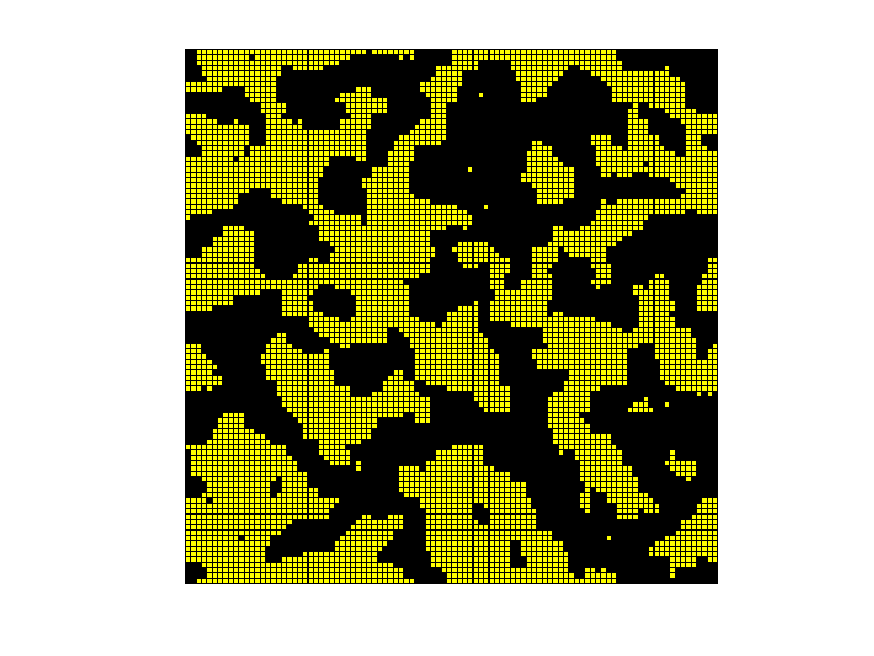
\includegraphics[width=0.8\linewidth]{../obtencion_resultados/a}
		\caption{Disposición para T=1 y 10$^5$ volteos}
		\label{fig:a}
	\end{figure}



	\begin{figure}[H]
		\centering
		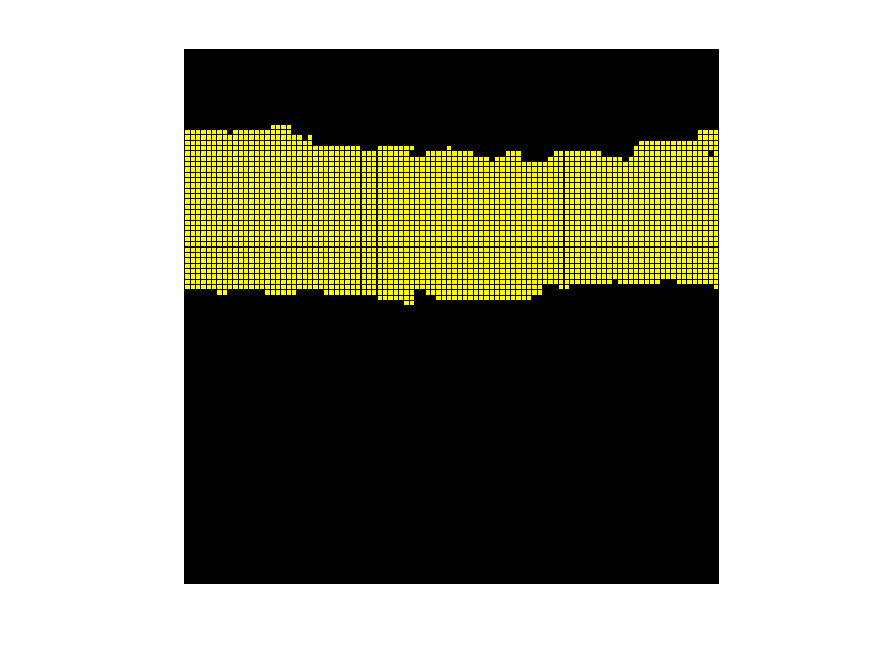
\includegraphics[width=0.8\linewidth]{../obtencion_resultados/b}
		\caption{Disposición para T=1 y 10$^8$ volteos}
		\label{fig:b}
	\end{figure}



	\begin{figure}[H]
		\centering
		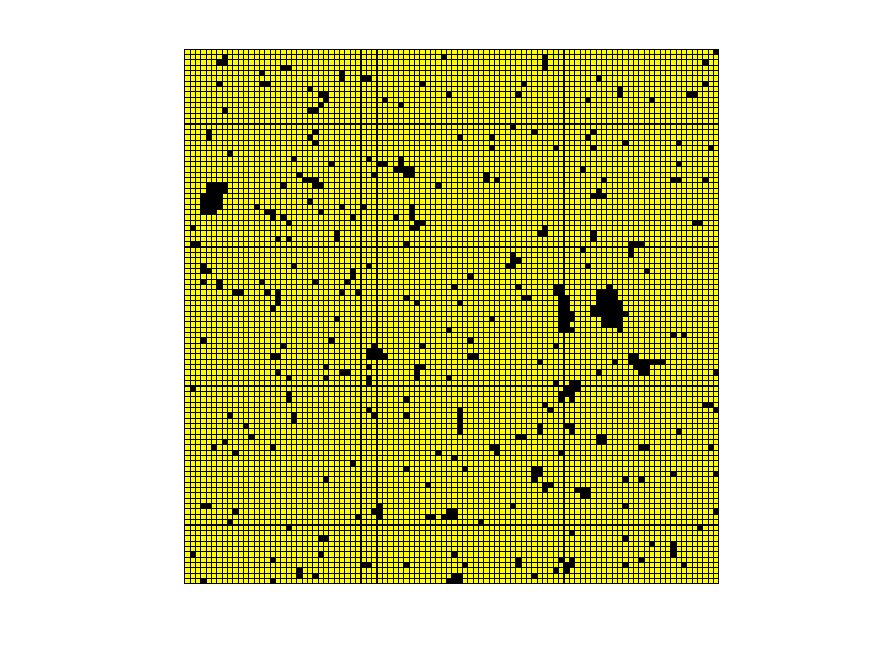
\includegraphics[width=0.8\linewidth]{../obtencion_resultados/c}
		\caption{Disposición para T=2 y 10$^8$ volteos}
		\label{fig:c}
	\end{figure}


	\begin{figure}[H]
		\centering
		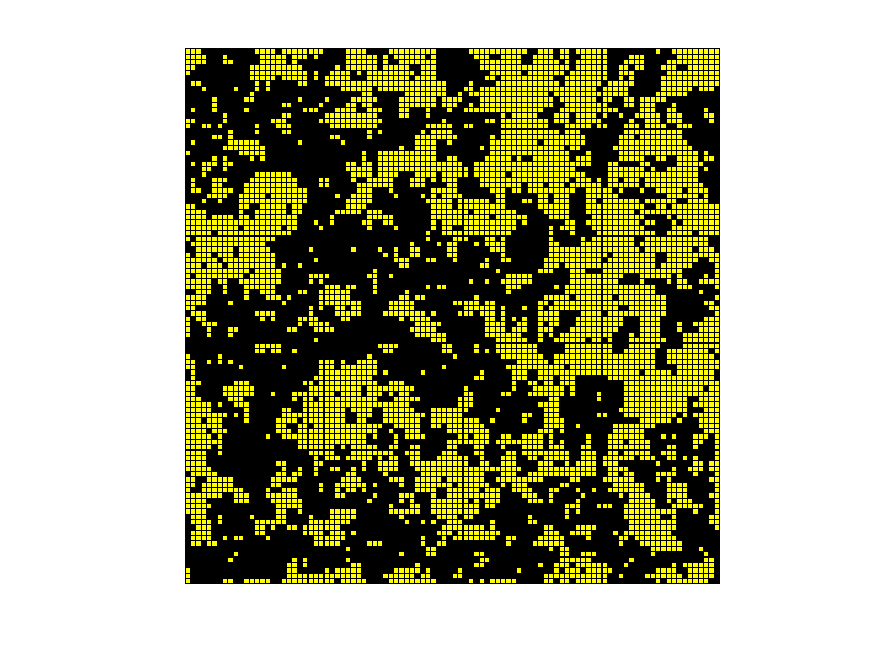
\includegraphics[width=0.8\linewidth]{../obtencion_resultados/d}
		\caption{Disposición para T=2.5 y 10$^8$ volteos}
		\label{fig:d}
	\end{figure}

	
	\subsection{Ejercicio 2}
	
	
	Para el siguiente ejercicio, modificamos el programa para que obtenga, a partir de una temperatura como parámetro, la evolución de la magnetización a lo largo de los pasos, guardando datos cada $10^4$ pasos. Obtenemos los datos de 6 temperaturas, y las representamos superpuestas en Matlab.
	
	
	
	\begin{figure}[H]
		\centering
		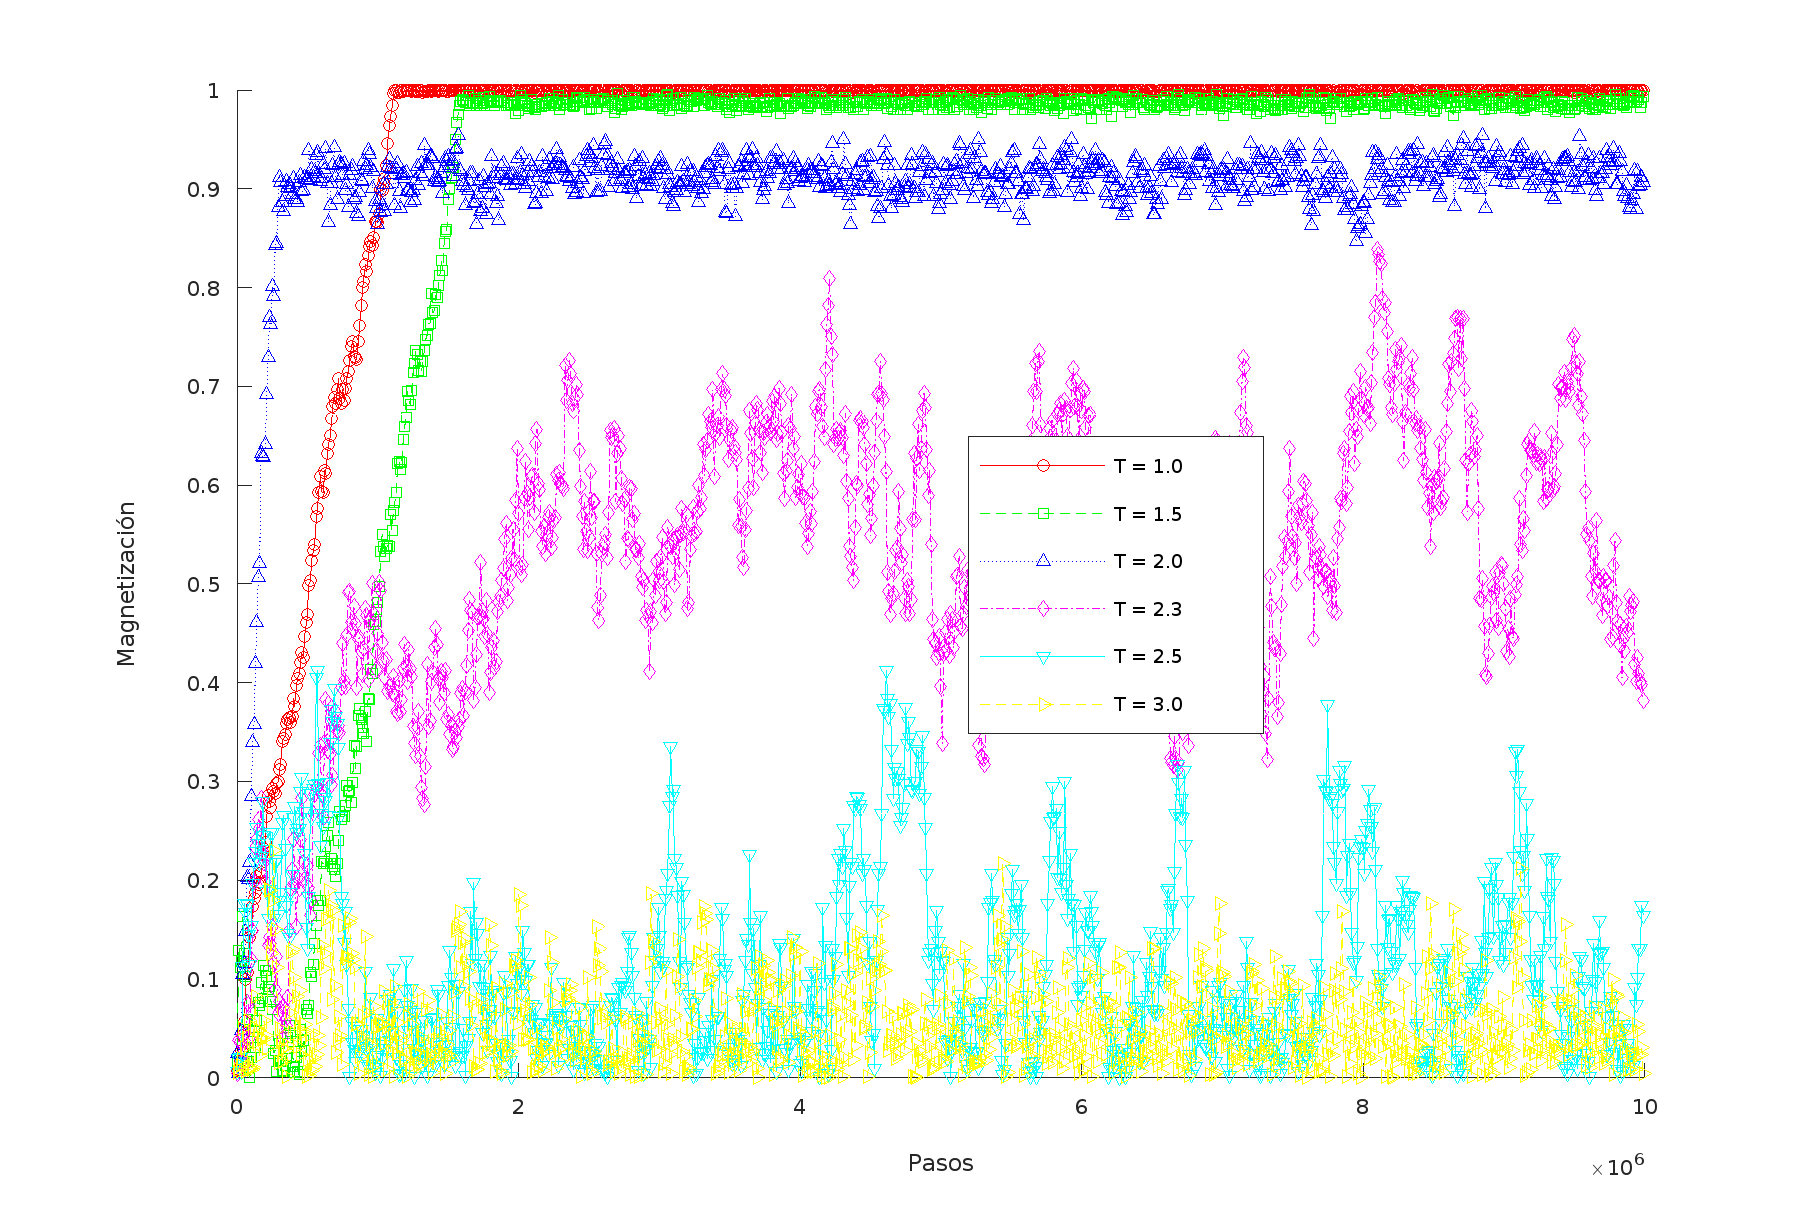
\includegraphics[width=1\linewidth]{../obtencion_resultados/grafica_ej2_marcadores_grande}
		\caption{Magnetización según la cantidad de pasos para distintas temperaturas}
		\label{fig:graficaej2}
	\end{figure}
	
	
	
	
	\subsection{Ejercicio 3}
	
	Finalmente, modificamos el programa para que obtenga la magnetización media de 5000 simulaciones para 11 temperaturas de 1,25 hasta 2,25 y las representamos junto a la expresión de Onsager.
	
	
	
	\begin{figure}[H]
		\centering
		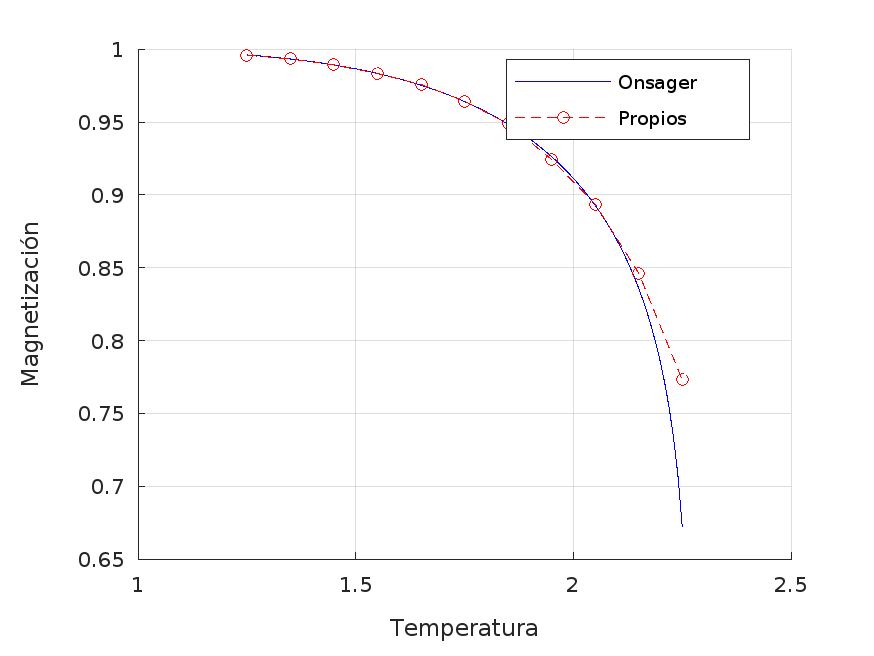
\includegraphics[width=0.9\linewidth]{../obtencion_resultados/grafica_ej3}
		\caption{Evolución de la magnetización media con la temperatura}
		\label{fig:graficaej3}
	\end{figure}
	
	
	


	\section{Análisis.}

\subsection{Ejercicio 1}


Para las dos primeras simulaciones, que tienen la misma temperatura, podemos ver en la Figura \ref{fig:a} cómo los spines están agrupados por cúmulos uniformes, pero todavía hay un equilibrio entre ambas orientaciones. En cambio, en la Figura \ref{fig:b}, los spines han terminado coincidiendo en una misma orientación en su mayoría. Aún queda una gran franja de distinta orientación, pero queda claro que las orientaciones tienden a converger hacia una de las dos. \\

La siguiente simulación, tomada a $T = 2$, podemos ver en la Figura \ref{fig:c} que también han terminado convergiendo, tal y como pasaba para $T = 1$, aunque en este caso parece ser menos homogéneo, vemos pequeños cúmulos de distinta orientación. Esta temperatura está más cerca de la temperatura crítica del sistema, lo que significa que la excitación térmica hace el sistema menos estable.\\


La última simulación, a $T = 2.5$, sobrepasa la temperatura crítica de $T_c = 2.27$. Vemos en la Figura \ref{fig:d} que la configuración no es uniforme. Se ven algunas agrupaciones, pero hay mucho más ruido del que había en el primer caso, ya que la alta temperatura genera una excitación mayor en los espines, por lo que es más probable que estos se volteen.\\

El algoritmo, cuando el cambio a realizar no es energéticamente favorable, genera un número aleatorio $r$ entre 0 y 1, y comprueba si es menor que la expresión de la probabilidad
\[ r < \exp\left(-\frac{\Delta H}{k_B T}\right)
\]
si lo es, realiza el volteo. Podemos ver que la expresión de la derecha aumenta con la temperatura, de modo que a mayor temperatura, más probable es que $r$ cumpla la condición y por tanto se voltee un espín energéticamente no favorable, en contra de la orientación mayoritaria de sus vecinos.


\subsection{Ejercicio 2}

En la Figura \ref{fig:graficaej2} vemos representada la evolución de la magnetización a lo largo de los pasos de simulación. Se puede observar mucha fluctuación, pero se puede ver con claridad como para las temperaturas más bajas, $T = 1$ y $T = 1,5$, la magnetización (el valor absoluto) llega a valores cercanos a 1 rápidamente. $T = 2$ sube más rápido, aunque esto parece ser fruto del azar, y se mantiene alrededor de $m = 0,9$, ya que su alta temperatura mantiene cierto nivel de inestabilidad que se opone a la uniformidad, como vimos en el ejercicio anterior para esta misma temperatura. \\

Para la temperatura $T = 2.3$, estamos justo en la temperatura crítica, y se puede observar mucha más fluctuación, sin llegar a decantarse por 1 ó 0. Pasado este punto crítico, vemos que para $T = 2.5$ el sistema mantiene la magnetización cerca de 0, aunque con más subidas que para $T = 3.0$, para la que solo llega a fluctuar hasta $|m| = 0,2$.


\subsection{Ejercicio 3}

En la Figura \ref{fig:graficaej3} vemos la representación de la magnetización media para distintas temperaturas superpuesta con la solución de Onsager. Podemos ver como se reduce con la temperatura coincidiendo especialmente en bajas temperaturas. La gráfica de la solución de Onsager cae en vertical cuando la temperatura se aproxima a $T_c$.

\section{Conclusión.}

Mediante una simulación en C y representaciones con Matlab, hemos podido comprobar el comportamiento a lo largo del tiempo de un modelo de Ising para distintas temperaturas, comprobando la validez de la solución de Onsager y el fenómeno de la temperatura crítica.


\section*{Anexo: sobre los programas y representaciones}

Quería hacer algunas anotaciones al códigos presentados. En primer lugar, planteé la opción de crear librerías con funciones recurrentes, pero para el alcance de estos ejercicios, encontré mucho más práctico simplemente copiar algunas funciones. También había algunos procesos que acababan teniendo que ser modificados de un ejercicio a otro, así que apenas he utilizado declaración de funciones y está todo principalmente en la función main().\\

En segundo lugar, para transferir los datos entre C y matlab, he utilizado \textit{.txt} de salida. He guardado los utilizados en el documento, de modo que pueden consultarlos y utilizarlos desde la carpeta \textit{'archivos\_de\_salida'} en el comprimido. También se incluyen los programas compilados (Linux).

	
\end{document}




